%%%%%%%%%%%%%%%%%%%%%%%%%%%%%%%%%%%%%%%%%
% Jacobs Portrait Poster
% LaTeX Template
% Version 1.0 (31/08/2015)
% (Based on Version 1.0 (29/03/13) of the landscape template
%
% Created by:
% Computational Physics and Biophysics Group, Jacobs University
% 
%https://teamwork.jacobs-university.de:8443/confluence/display/CoPandBiG/LaTeX+Poster
% 
% Further modified by:
% Nathaniel Johnston (nathaniel@njohnston.ca)
%
% Portrait version by:
% John Hammersley
%
% The landscape version of this template was downloaded from:
% http://www.LaTeXTemplates.com
%
% License:
% CC BY-NC-SA 3.0 (http://creativecommons.org/licenses/by-nc-sa/3.0/)
%
%%%%%%%%%%%%%%%%%%%%%%%%%%%%%%%%%%%%%%%%%

%----------------------------------------------------------------------------------------
%	PACKAGES AND OTHER DOCUMENT CONFIGURATIONS
%----------------------------------------------------------------------------------------

\documentclass[final,noamsthm]{beamer}

\usepackage[scale=1.24]{beamerposter} % Use the beamerposter package for laying out the poster

% Define math environment
\newtheorem{theorem2}{Theorem}
\newtheorem{corollary2}[theorem2]{Corollary}
\newtheorem{lemma2}[theorem2]{Lemma}
\newtheorem{definition2}[theorem2]{Definition}

\usepackage{enumerate}
\usepackage{pdfpages}


\usetheme{confposter} % Use the confposter theme supplied with this template

\definecolor{primary} {HTML}{0088cf}
\definecolor{secondary} {HTML}{ff213e}

\setbeamercolor{block title}{fg=primary,bg=white} % Colors of the block 
%titles
\setbeamercolor{block body}{fg=black,bg=white} % Colors of the body of blocks
%\setbeamercolor{block alerted title}{fg=white,bg=secondary!90} % Colors 
%%of 
%the highlighted block titles
%\setbeamercolor{block alerted body}{fg=black,bg=secondary!10} % Colors of 
%the body of highlighted blocks

% set colors for itemize/enumerate
\setbeamercolor{item}{fg=primary}
\setbeamercolor{item projected}{fg=white,bg=primary}

%-----------------------------------------------------------
% Define the column widths and overall poster size
% To set effective sepwid, onecolwid and twocolwid values, first choose how many columns you want and how much separation you want between columns
% In this template, the separation width chosen is 0.024 of the paper width and a 4-column layout
% onecolwid should therefore be (1-(# of columns+1)*sepwid)/# of columns e.g. (1-(4+1)*0.024)/4 = 0.22
% Set twocolwid to be (2*onecolwid)+sepwid = 0.464
% Set threecolwid to be (3*onecolwid)+2*sepwid = 0.708

\newlength{\sepwid}
\newlength{\onecolwid}
\newlength{\twocolwid}
\newlength{\threecolwid}
%\setlength{\paperwidth}{23.4in} % A1
%\setlength{\paperheight}{33.1in} % A1
\setlength{\paperwidth}{33.1in} % A0
\setlength{\paperheight}{46.8in} % A0
\setlength{\sepwid}{0.024\paperwidth} % Separation width (white space) between columns
\setlength{\onecolwid}{0.301\paperwidth} % Width of one column
\setlength{\twocolwid}{0.627\paperwidth} % Width of two columns
\setlength{\threecolwid}{\paperwidth} % Width of three columns
\setlength{\topmargin}{-0.5in} % Reduce the top margin size
%-----------------------------------------------------------

\usepackage{graphicx}  % Required for including images

\usepackage{booktabs} % Top and bottom rules for tables

%----------------------------------------------------------------------------------------
%	TITLE SECTION 
%----------------------------------------------------------------------------------------

\title{Does the GDPR protect my identity in mobile apps?} % Poster title

\author{Konrad Kollnig - Max van Kleek (Supervisor)} % 
%Author(s)

\institute{konrad.kollnig@cs.ox.ac.uk - Computer Science @ University of 
Oxford} % Institution(s)

%----------------------------------------------------------------------------------------

\begin{document}

\addtobeamertemplate{block end}{}{\vspace*{2ex}} % White space under blocks
\addtobeamertemplate{block alerted end}{}{\vspace*{2ex}} % White space under highlighted (alert) blocks

\setlength{\belowcaptionskip}{2ex} % White space under figures
\setlength\belowdisplayshortskip{2ex} % White space under equations

\begin{frame}[t] % The whole poster is enclosed in one beamer frame

\begin{center}
	\centering
	\LARGE
	What are the provisions of the GDPR?
\end{center}


\begin{columns}[t]
	
	\begin{column}{\sepwid}\end{column} % Empty spacer column
	
	\begin{column}{\onecolwid} % The first column
		\begin{block}{Introduction to GDPR}
			The introduction of the EU's General Data Protection 
			Regulation (GDPR) in 2018 is supposed to change the handling 
			of data 
			fundamentally. It does so by:
			\begin{itemize}
				\item Introducing a common standard across the EU,
				\item Defining personal data more rigorously,
				\item Tightening the conditions for collecting personal 
				data, through \textit{affirmative consent}.
			\end{itemize}
		\end{block}
		
	\end{column}
	\begin{column}{\sepwid}\end{column} % Empty spacer column
	
	\begin{column}{\onecolwid} % The second column
		\begin{block}{What is personal data?}
			\textbf{Definition:}
			\textit{'Personal data'} means any information relating to an 
			identified or identifiable natural person (\textit{'data 
			subject'}).
		
			The term \textit{relates} makes clear that there must be means 
			to identify an individual from the data.
			
			Collection of personal data is \textit{lawful} under GDPR, if 
			one of six legal bases is established.
			The vast majority of mobile apps relies on the legal 
			basis
			\textit{legitimate interest} or \textit{affirmative 
			consent}.
		\end{block}
	\end{column}
	\begin{column}{\sepwid}\end{column} % Empty spacer column
	
	\begin{column}{\onecolwid} % The third column
		\begin{block}{What rights does a user have?}
			The GDPR specifies eight rights of the data subject, for
		 before and after the collection of data:
			\vspace{-0.5cm}
			\begin{columns}
				\begin{column}{0.5\textwidth}
					\begin{itemize}
						\small
						\item \textit{Right to be informed}
						\item Right of access
						\item Right to rectification
						\item Right to erasure
					\end{itemize}
				\end{column}
				\begin{column}{0.5\textwidth}
					\begin{itemize}
						\small
						\item Right to restrict processing
						\item Right to data portability
						\item Right to object
						\item Rights w.r.t. automated decision-making + 
						profiling
					\end{itemize}
				\end{column}
			\end{columns}
			\vspace{0.5cm}
			$\Rightarrow$The app user must \textbf{be informed} about the 
			privacy 
			policies \textbf{at 
				the time of data collection}.
		\end{block}
	\end{column}

	\begin{column}{\sepwid}\end{column} % Empty spacer column
\end{columns}

\begin{center}
    \centering
    {\LARGE
    Opening an app's privacy policy must be without data collection, 
    but..}
	\vspace{0.5cm}
	{\\ \large
	..that's not what you find for the top 26 771 apps.}
	% Three arguments for this interpretation:
	% 1. From a technical perspective, there is data collected before the 
	%data subject can see the policies
	% 2. The GDPR is all about choice. Therefore, the user should have a 
	%choice about data collection, and be able to freely learn about the 
	%conditions that apply.
\end{center}

\begin{columns}[t]

\begin{column}{\sepwid}\end{column} % Empty spacer column

\begin{column}{\onecolwid} % The first column

\begin{block}{Tracking by revenue and recency}
	\begin{figure}
		\label{fig:rev}
		\includegraphics[width=\textwidth]{figures/by_collection.pdf}
		\caption{ \ (\textasciitilde7600 
			apps/collection)
		If any trackers are used, then \textbf{analytics almost always} is.
		Whilst the policies of
		paid apps bring trackers less likely than free ones, they 
		often provide no privacy policy. Having no policy might 
		\textbf{indicate no data collection}.
		GDPR information requests confirm this, but less than 
		half of the companies replied ($n=53$). }
	\end{figure}
\end{block}

\end{column}
\begin{column}{\sepwid}\end{column} % Empty spacer column

\begin{column}{\onecolwid} % The second column
\begin{block}{Tracking by platform}
	\begin{figure}
		\includegraphics[width=\textwidth]{figures/by_platform.pdf}
		\caption{ \ (\textasciitilde4000 
			apps/platform)  Almost \textbf{no differences} in privacy 
			policy 
		tracking between the platforms are noticeable. iOS shows slightly 
		higher number 
		of apps 
			without privacy policies, which might be an indicator 
			of \textbf{no 
			data collection}, see Figure~\ref{fig:rev}.}
	\end{figure}
\end{block}
\end{column}
\begin{column}{\sepwid}\end{column} % Empty spacer column

\begin{column}{\onecolwid} % The third column
	\begin{block}{Tracking by store country}
		\begin{figure}
			\includegraphics[width=\textwidth]{figures/by_country.pdf}
			\caption{ \ (\textasciitilde7600 
				apps/country) The \textbf{differences} in privacy policy 
			tracking between 
			the countries of the 
			app 
			store 
			charts are \textbf{marginal}. Only Poland (PL) shows a higher 
			number of apps without privacy policies and fewer trackers 
			overall.}
		\end{figure}
	\end{block}
\end{column}


\begin{column}{\sepwid}\end{column} % Empty spacer column

\end{columns}

\begin{center}
	\centering
	{\LARGE
		Oh wow, why not just exert my GDPR rights?}
\end{center}

\begin{columns}[t]
	
	\begin{column}{\sepwid}\end{column} % Empty spacer column
	
	\begin{column}{\onecolwid} % The first column
		\begin{block}{Options to exert rights}
			\begin{itemize}
				\item Send an \textbf{email} (GDPR 
				Request).				
				Problem: Low reply rate. I tried, just as many others.
				\item Make a \textbf{complaint} to the data authorities.
				Problem: Scope. There are some 12 million app 
				developers (Source: Evans Data Corp.).
				\item Take \textbf{legal action}. Problem: Feasibility. 
				What user would do this?
			\end{itemize}
		\end{block}
		\begin{block}{Conclusions}
			\begin{itemize}
				\item First \textbf{large-scale study}, comparing 
				Android/iOS apps with 
				free/paid ones.
				\item Mobile users are \textbf{heavily tracked}, as 
				numerous studies found and confirmed herein; paid and iOS 
				apps might be slightly better.
				\item It is \textbf{difficult to take action} for regular 
				app 
				users. The GDPR has \textbf{failed} in this sense. 
			\end{itemize} 
		\end{block}
		
	\end{column}
	\begin{column}{\sepwid}\end{column} % Empty spacer column
	
	\begin{column}{\onecolwid} % The second column
		\begin{block}{Next steps}
			\begin{itemize}
				\item Investigation of
				correlation between \textbf{trackers in 
				apps} and in their policies.
				\item Derivation of metric to identify 
				\textbf{most-invasive apps}, so as to inform app users.
				\item Development of platform for \textbf{easy and 
				effective enforcement} of GDPR rights.
			\end{itemize}
		\end{block}
	
		\begin{alertblock}{Join the mailing list}
			\centering
			\textbf{Be first to get access} to our privacy tools:
			\\ \includegraphics[width=0.38\textwidth]{figures/email_qr.eps}
			\\ Or, email to: konrad.kollnig@cs.ox.ac.uk
		\end{alertblock}
	\end{column}
	\begin{column}{\sepwid}\end{column} % Empty spacer column
	
	\begin{column}{\onecolwid} % The third column
		\begin{block}{Aim: Privacy Mission Control}
			\begin{figure}
				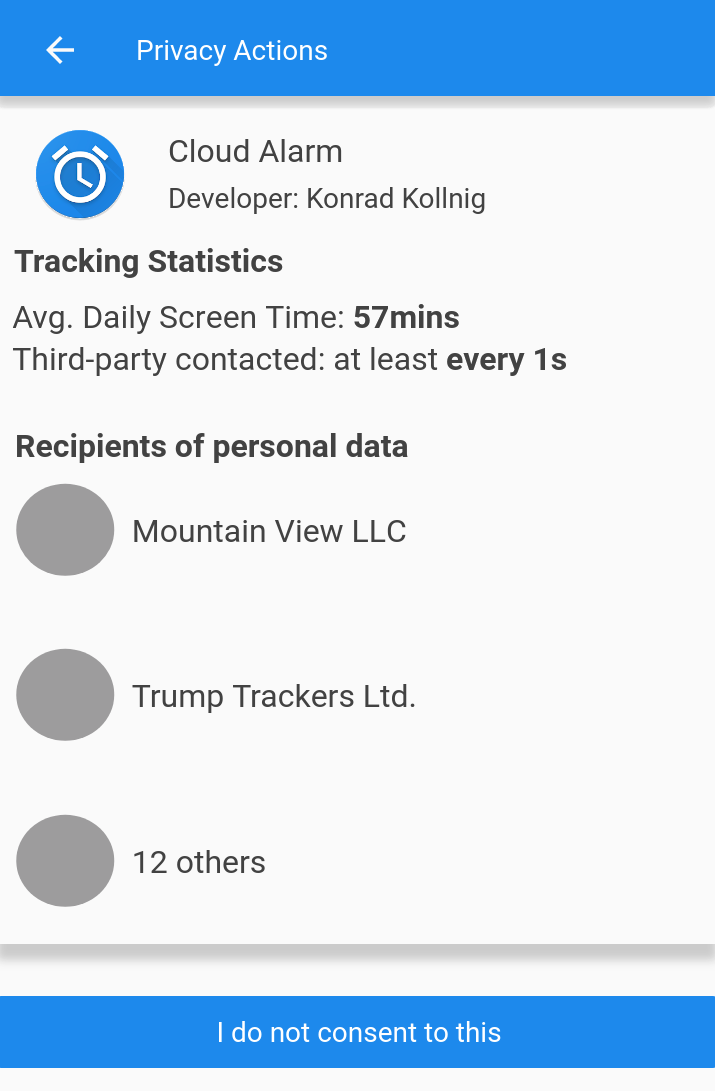
\includegraphics[width=0.77\textwidth]{figures/mock.png}
			\end{figure}
		\end{block}
	\end{column}
	
	
	\begin{column}{\sepwid}\end{column} % Empty spacer column
	
\end{columns}

\end{frame} % End of the enclosing frame

\end{document}
